\documentclass[conference]{IEEEtran}
\IEEEoverridecommandlockouts
\usepackage[utf8]{inputenc}
\usepackage[T1]{fontenc}
\usepackage{cite}
\usepackage{amsmath,amssymb,amsfonts}
\usepackage{algorithmic}
\usepackage{graphicx}
\usepackage{textcomp}
\usepackage{xcolor}
\usepackage{listings}
\lstset{
  language=Python,
  basicstyle=\ttfamily\small,
  keywordstyle=\bfseries,
  showstringspaces=false,
  breaklines=true,
  frame=single,
  columns=fullflexible
}
\def\BibTeX{{\rm B\kern-.05em{\sc i\kern-.025em b}\kern-.08em
    T\kern-.1667em\lower.7ex\hbox{E}\kern-.125emX}}
\begin{document}

% TODO (grupo): titulo ainda nao aprovado pelo grupo -- reflete o pivo para adaptabilidade
\title{Spino: uma arquitetura modular de baixo custo para telemetria adaptável a múltiplos casos de uso}

\author{
\IEEEauthorblockN{Arthur de Morais Marques}
\IEEEauthorblockA{\textit{Laboratório de Tecnologia (LabTech)} \\
\textit{IFSP -- Câmpus Caraguatatuba}\\
Caraguatatuba, Brasil \\
arthur.morais@aluno.ifsp.edu.br}
\and
\IEEEauthorblockN{Kauan Edson Leonel Lira}
\IEEEauthorblockA{\textit{Laboratório de Tecnologia (LabTech)} \\
\textit{IFSP -- Câmpus Caraguatatuba}\\
Caraguatatuba, Brasil \\
leonel@ifspcaragua.net}
\and
\IEEEauthorblockN{Daniel Patrick de Morais}
\IEEEauthorblockA{\textit{Laboratório de Tecnologia (LabTech)} \\
\textit{IFSP -- Câmpus Caraguatatuba}\\
Caraguatatuba, Brasil \\
% TODO (Daniel): confirmar e-mail
danielmorais@ifspcaragua.net}
\and
\IEEEauthorblockN{Ederson Rafael Wagner}
\IEEEauthorblockA{\textit{Laboratório de Tecnologia (LabTech)} \\
\textit{IFSP -- Câmpus Caraguatatuba}\\
Caraguatatuba, Brasil \\
% TODO (Ederson): confirmar e-mail
erwagner@ifsp.edu.br}
}

\maketitle

% TODO (grupo): rascunho de abstract refletindo o enfoque em arquitetura/adaptabilidade -- revisar
\begin{abstract}
Sistemas de baixo custo para aquisição remota de dados precisam conciliar confiabilidade, comunicação sem fio e adaptabilidade a diferentes aplicações. Este trabalho apresenta o Spino, uma arquitetura modular composta por três módulos -- aquisição de campo, processamento de borda e supervisão local, e centralização web das regras de negócio -- projetada para ser reconfigurável entre diferentes domínios de sensoriamento remoto. Descreve-se em detalhe a arquitetura de cada módulo e o estado atual de sua implementação, empregando como estudo de caso o monitoramento de ensaios de carga em competições de pontes de palito. No estágio atual, o Módulo 1 opera de forma autônoma e completa; o Módulo 2 recebe, valida e processa os dados, disponibilizando parte deles em uma interface de exibição local; e o Módulo 3 já implementa cadastro de equipes e persistência, restando concluir a integração entre os módulos de borda e supervisão para a operação de ponta a ponta.
\end{abstract}

\begin{IEEEkeywords}
sensoriamento remoto, telemetria, arquitetura modular, computação de borda, comunicação por radiofrequência
\end{IEEEkeywords}

\section{Introdução}
O sensoriamento remoto -- a aquisição de uma grandeza física sem contato direto com o objeto observado \cite{quartaroli2014} -- é empregado em aplicações que vão do monitoramento ambiental ao acompanhamento de ensaios estruturais, apoiando atividades de supervisão, registro histórico, emissão de alertas e tomada de decisão conforme as regras de cada aplicação. Soluções desenvolvidas para uma finalidade específica tendem, no entanto, a acoplar sensores, processamento, comunicação e interface de acompanhamento em um único sistema dedicado.

Esse acoplamento dificulta a adaptação do sistema quando se altera a grandeza monitorada, os requisitos de processamento ou o contexto de uso: cada nova aplicação tende a exigir o redesenho de partes que, em princípio, poderiam ser reaproveitadas, elevando o custo e o tempo de desenvolvimento -- uma barreira especialmente relevante em contextos de baixo orçamento, como projetos acadêmicos e institucionais.

Sistemas de aquisição de dados baseados em microcontroladores de baixo custo são amplamente empregados para atender a essa necessidade \cite{vidalpardo2018,njoku2025,elabd2017}. Em geral, no entanto, esses sistemas são projetados para uma aplicação específica, com a lógica de processamento, a comunicação e a interface de acompanhamento integradas ao mesmo hardware -- o que os torna eficazes para o caso-alvo, mas pouco reaproveitáveis quando a grandeza monitorada ou o cenário de uso mudam.

Para lidar com essa limitação, este trabalho apresenta o Spino, uma arquitetura modular organizada em três módulos com responsabilidades desacopladas: aquisição de campo, processamento de borda e supervisão web. Essa separação, detalhada na Seção II, permite que cada módulo seja adaptado, substituído ou testado de forma independente, favorecendo o reaproveitamento da arquitetura em diferentes domínios de sensoriamento remoto.

Como instanciação da arquitetura, considera-se o Concurso de Pontes de Palito do curso de Engenharia Civil do Instituto Federal de São Paulo (IFSP), campus Caraguatatuba, no qual as estruturas construídas pelos competidores são submetidas a cargas crescentes até a ruptura, com o objetivo de determinar a carga máxima suportada por cada ponte. Nesse cenário, o Módulo 1 é empregado para adquirir os dados de carga da estrutura durante o ensaio, enquanto os módulos subsequentes tratam, transmitem e organizam essas informações no contexto do evento.

Este trabalho tem como objetivo detalhar essa arquitetura e descrever sua instanciação para a aquisição e a transmissão de dados de carga no estudo de caso adotado. O Módulo 1 é apresentado em sua implementação atual, plenamente funcional; os Módulos 2 e 3 são descritos como componentes da arquitetura proposta para processamento de borda, persistência, supervisão e aplicação de regras de negócio, com o estado de implementação de cada um discutido ao longo do texto.

Para isso, estrutura-se o Módulo 1 para aquisição contínua de dados de carga por meio de sensores, microcontrolador e comunicação por radiofrequência; implementa-se o Módulo 2 como camada de computação de borda, responsável por receber, pré-processar, armazenar temporariamente e exibir localmente os dados, encaminhando-os ao servidor por requisições HTTP; e projeta-se o Módulo 3 como plataforma web para persistência, distribuição de atualizações em tempo real e centralização das regras de negócio da competição. Quando os dados coletados permitirem, avalia-se ainda, em bancada, a correspondência entre cargas de referência e leituras recebidas, a entrega de pacotes e o atraso de comunicação.

\section{Arquitetura da Plataforma Spino}

\subsection{Visão Geral}
A arquitetura do Spino organiza-se em três módulos com responsabilidades bem delimitadas, descritos nas subseções seguintes: aquisição de campo (Módulo 1), processamento de borda e supervisão local (Módulo 2) e centralização das regras de negócio em uma plataforma web (Módulo 3). Essa divisão permite que cada módulo evolua, seja substituído ou testado de forma independente, sem exigir alterações nos demais. A Figura~\ref{fig:arquitetura} apresenta a visão geral da arquitetura, incluindo os componentes internos de cada módulo e os pontos de comunicação entre eles.

\begin{figure*}[t]
\centering
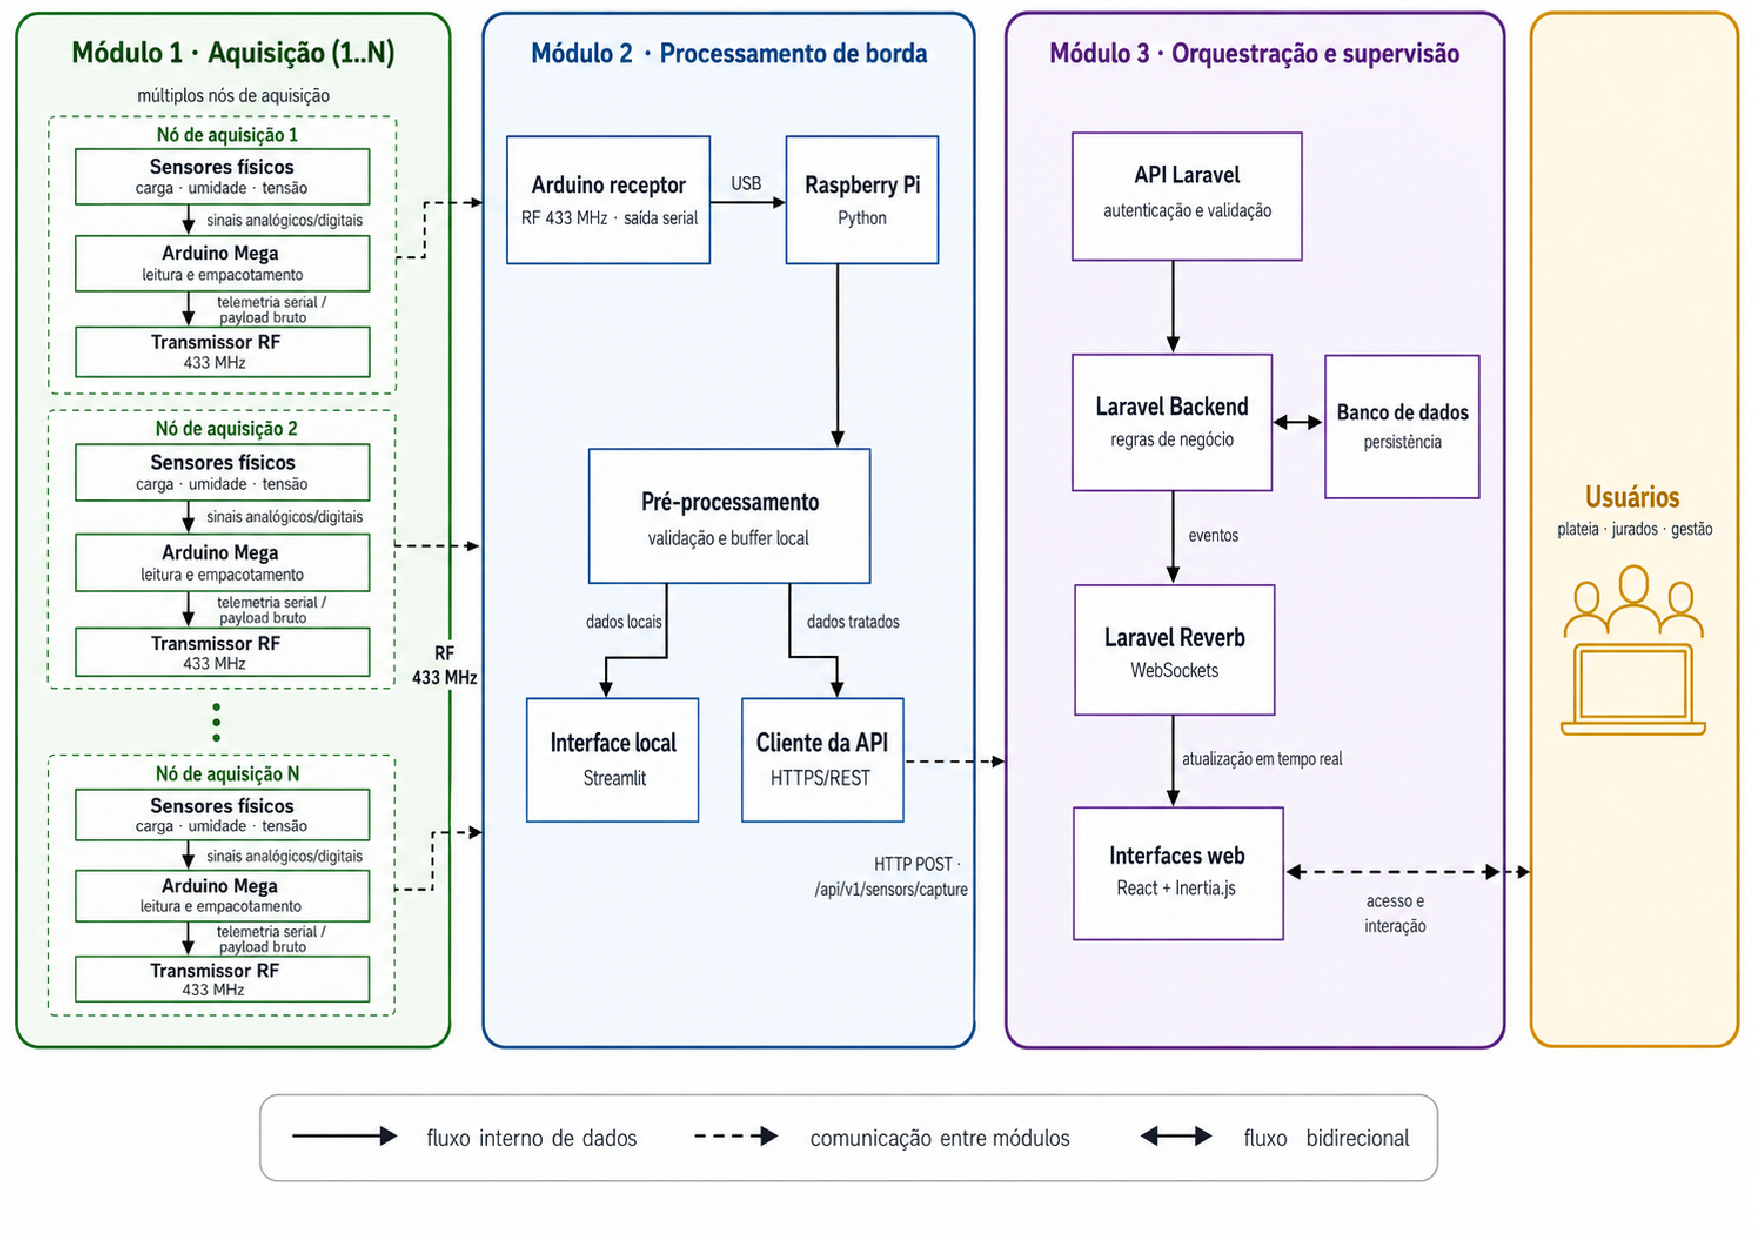
\includegraphics[width=0.85\textwidth]{figuras/arquitetura_spino_atualizada.pdf}
\caption{Visão geral da arquitetura do Spino, com os três módulos e seus componentes internos.}
\label{fig:arquitetura}
\end{figure*}

\subsection{Módulo 1 --- Sensoriamento, processamento e transmissão}

O Módulo 1 constitui a unidade de campo da arquitetura Spino,
sendo responsável pela interação direta com os sensores e demais
componentes instalados no ambiente ou na estrutura monitorada.
Suas principais funções são adquirir as grandezas físicas de
interesse, realizar o processamento inicial das leituras,
acompanhar as condições de operação, organizar as informações
segundo o protocolo de comunicação do Spino e transmitir o quadro
resultante ao Módulo 2 por meio de comunicação sem fio
\cite{ouldzira2019,vidalpardo2018,njoku2025}.

A unidade central do módulo pode ser composta por um
microcontrolador escolhido conforme os requisitos da aplicação.
Neste projeto, foi utilizado um Arduino Mega em razão da
quantidade de entradas e saídas disponíveis, da presença de
múltiplas interfaces seriais e da compatibilidade com os sensores
e módulos de comunicação empregados
\cite{vidalpardo2018,njoku2025,elabd2017,arduinodocs}.
Entretanto, essa escolha não é fixa, podendo o componente ser
substituído por outro microcontrolador que atenda aos requisitos
da aplicação.

A configuração dos sensores conectados ao Módulo 1 depende do
caso de uso em que o Spino é empregado. No estudo de caso das
pontes de palito, sensores são utilizados para adquirir a carga
aplicada e uma medida associada à flexão da estrutura,
representada pela deflexão observada no ponto instrumentado. O
módulo também acompanha o nível de alimentação e o tempo
transcorrido do ensaio. Esses dados correspondem aos campos de
carga máxima, carga atual, deflexão, tempo, nível de bateria e
estado de operação apresentados na
Tabela~\ref{tab:protocolo}.

\begin{table}[htbp]
    \caption{Estrutura do quadro do protocolo de comunicação
    do Spino}
    \label{tab:protocolo}
    \centering
    \footnotesize
    \renewcommand{\arraystretch}{1.05}
    \begin{tabular}{|c|c|c|p{3.25cm}|}
        \hline
        \textbf{Pos.} &
        \textbf{Campo} &
        \textbf{Car.} &
        \textbf{Descrição} \\
        \hline
        0--2 & \texttt{INI} & 3 &
        Delimitador de início \texttt{***} \\
        \hline
        3--5 & \texttt{BAT} & 3 &
        Nível de bateria \\
        \hline
        6--9 & \texttt{CM} & 4 &
        Carga máxima registrada \\
        \hline
        10--13 & \texttt{CA} & 4 &
        Carga atual \\
        \hline
        14--16 & \texttt{DEF} & 3 &
        Deflexão associada à flexão da ponte \\
        \hline
        17--20 & \texttt{TEM} & 4 &
        Tempo transcorrido do ensaio \\
        \hline
        21 & \texttt{F} & 1 &
        Flag de operação, 0 ou 1 \\
        \hline
        22--23 & \texttt{CHK} & 2 &
        Checksum do quadro \\
        \hline
        24--26 & \texttt{FIM} & 3 &
        Delimitador de fim \texttt{\#\#\#} \\
        \hline
    \end{tabular}

    \vspace{0.1cm}
    \parbox{0.98\columnwidth}{
        \footnotesize
        Os campos numéricos são transmitidos como cadeias de
        caracteres de largura fixa. Quando necessário, são
        acrescentados zeros à esquerda. As unidades e escalas
        empregadas devem ser definidas de forma idêntica no
        transmissor e no receptor.
    }
\end{table}

A organização do Módulo 1 não está limitada a essas grandezas.
Outros sensores podem ser integrados, desde que suas interfaces
sejam compatíveis com o microcontrolador e suas leituras sejam
tratadas pelo software embarcado
\cite{vidalpardo2018,njoku2025}.

Após a aquisição, os dados passam por uma etapa de processamento
local. Essa etapa pode envolver conversão de unidades, aplicação
de fatores de calibração, filtragem de oscilações, comparação com
valores anteriores e identificação de condições específicas da
aplicação \cite{vidalpardo2018,njoku2025}. No estudo de caso, o
sistema mantém, entre outras informações, a carga atual, a maior
carga observada durante o ensaio, a deflexão da estrutura e o
tempo transcorrido.

Depois de processadas, as informações são organizadas segundo o
protocolo de comunicação do Spino. Um protocolo estabelece as
regras relacionadas ao formato, ao significado e à ordem das
mensagens trocadas entre as entidades comunicantes
\cite{tanenbaum2011}. No Spino, essas regras definem o
comprimento do quadro, a posição ocupada por cada informação,
os delimitadores de início e fim e o mecanismo utilizado para a
verificação de integridade.


Os identificadores apresentados nessa representação são apenas
simbólicos e não são transmitidos juntamente com os valores. O
receptor identifica cada informação de acordo com sua posição no
quadro. Os campos \texttt{INI} e \texttt{FIM} delimitam a
mensagem; \texttt{BAT} representa o nível de bateria;
\texttt{CM} e \texttt{CA} representam, respectivamente, a carga
máxima e a carga atual; \texttt{DEF} representa a deflexão
associada à flexão da estrutura; \texttt{TEM} representa o tempo
de ensaio; \texttt{F} indica o estado de operação; e
\texttt{CHK} contém o checksum. A
Tabela~\ref{tab:protocolo} apresenta as posições reservadas a cada
campo.

A comunicação entre os Módulos 1 e 2 é realizada por
radiofrequência na faixa de 433~MHz \cite{ouldzira2019}. Em
cada ciclo de funcionamento, o microcontrolador realiza a
leitura dos sensores, atualiza o tempo e as variáveis de
operação, processa os valores adquiridos, constrói o quadro
segundo o protocolo de comunicação e solicita sua transmissão.
Esse ciclo é executado periodicamente, permitindo a atualização
das informações ao longo do ensaio.

A separação entre aquisição, processamento, comunicação e
supervisão constitui um dos princípios da arquitetura Spino. O
Módulo 1 concentra as funções diretamente relacionadas à
instrumentação e ao tratamento inicial das grandezas físicas. O
Módulo 2 realiza a recepção, a validação e o processamento de
borda, enquanto o Módulo 3 concentra a persistência, as regras
de negócio e a supervisão web. Dessa forma, alterações nas
interfaces de supervisão não exigem modificações diretas nos
sensores, desde que sejam preservadas as interfaces de
comunicação entre os módulos.

Essa organização possibilita a utilização do Módulo 1 em
diferentes projetos. Em um pluviômetro, por exemplo, o módulo
pode receber dados de um sensor de precipitação e processar
informações como quantidade de basculamentos, volume acumulado
e intensidade da chuva. Em uma estação ambiental, pode integrar
sensores de temperatura, umidade e pressão. Já em aplicações
estruturais, pode receber dados de células de carga, sensores de
deformação ou deslocamento e outros dispositivos de
instrumentação. A integração de diferentes sensores em sistemas
de aquisição baseados em Arduino é demonstrada em aplicações
experimentais que envolvem a coleta e o processamento simultâneo
de diferentes grandezas físicas
\cite{vidalpardo2018,njoku2025}.

Embora a configuração empregada neste estudo esteja relacionada
ao monitoramento de pontes de palito, o Módulo 1 foi concebido
como uma unidade configurável de aquisição, processamento e
comunicação. Sua adaptação a outras aplicações exige
principalmente a substituição dos sensores, a alteração das regras
de processamento e a redefinição dos campos específicos do
protocolo, preservando-se o fluxo geral de aquisição, tratamento e
transmissão dos dados.

\subsection{Módulo 2 --- Processamento de borda e supervisão local}
O Módulo 2 representa a camada intermediária de processamento de borda (\textit{edge computing}) da arquitetura Spino, atuando como elo entre os módulos de aquisição (Módulo 1) e o sistema de supervisão (Módulo 3). Sua função é receber os protocolos de comunicação transmitidos por uma ou mais unidades do Módulo 1 operando simultaneamente, validar sua integridade, interpretar os campos da mensagem, organizar os dados recebidos e encaminhá-los ao servidor de supervisão.

A plataforma computacional principal do Módulo 2 é um Raspberry Pi 3B+, escolhido por oferecer capacidade de processamento e conectividade de rede suficientes a baixo custo. Essa escolha, entretanto, não é obrigatória: a arquitetura admite qualquer computador embarcado capaz de executar um sistema operacional, interpretar os dados recebidos e comunicar-se com o servidor de supervisão por meio de protocolos de rede.

A recepção dos sinais de radiofrequência em 433 MHz é realizada diretamente pelo Raspberry Pi, por meio de um módulo receptor RF conectado ao dispositivo. Um processo em execução no Raspberry Pi monitora continuamente esse módulo, identificando novas mensagens, realizando sua leitura e encaminhando-as às etapas seguintes de processamento.

O emprego do processamento de borda nesta camada tem papel central na arquitetura Spino: ao concentrar validações e tratamentos próximos da origem dos dados, essa abordagem reduz a carga computacional do servidor central, diminui o tráfego de informações desnecessárias em direção à supervisão e aumenta a robustez do sistema frente a instabilidades pontuais de rede \cite{shi2016}.

Após a recepção de cada mensagem, o software executado no Raspberry Pi realiza as etapas necessárias para interpretar o quadro recebido: identifica os delimitadores de início e fim, valida sua estrutura, separa os campos do quadro e converte os valores recebidos para os tipos de dados correspondentes. Em seguida, verifica a integridade da mensagem por meio do mecanismo de checksum já definido no protocolo do Módulo 1 \cite{tanenbaum2011}, descartando quadros inválidos e tratando eventuais erros de comunicação antes de preparar os dados para as etapas seguintes. Essa validação prévia evita o armazenamento de informações corrompidas ou inconsistentes no sistema de supervisão. 

Além dessas validações, o Módulo 2 pode incorporar funções adicionais de pré-processamento, como filtragem de mensagens duplicadas, controle da frequência de envio, agregação de leituras, identificação de falhas de comunicação, registro de eventos locais e armazenamento temporário dos dados em situações de indisponibilidade do servidor. Essas funções tornam o sistema mais resiliente diante de falhas temporárias de conectividade.

Os dados processados também alimentam uma interface de exibição em tempo real, implementada em Python com a biblioteca Streamlit, que apresenta as leituras recebidas e permite o acompanhamento contínuo do ensaio diretamente no ponto de supervisão local, de forma independente da disponibilidade do Módulo 3.

Esse arranjo reforça o princípio de desacoplamento entre a comunicação física e a aplicação: o Módulo 2 isola por completo o protocolo de radiofrequência da infraestrutura web, permitindo alterar o método de comunicação com o servidor de supervisão sem qualquer modificação no funcionamento do Módulo 1. Essa separação também facilita a realização de testes individuais de cada módulo, simplifica a manutenção e favorece a evolução independente da arquitetura.

Após todas as validações, os dados processados são encapsulados em uma estrutura adequada -- como JSON -- e encaminhados ao backend por meio de requisições HTTP REST, utilizando o endpoint disponibilizado pelo Módulo 3 para essa finalidade. No estágio atual do projeto, essa etapa de integração ainda está em desenvolvimento, de modo que o encaminhamento ao Módulo 3 é descrito aqui como arquitetura proposta.

A modularidade da arquitetura Spino permite ainda que o Módulo 2 seja adaptado para outras tecnologias de comunicação além da radiofrequência em 433 MHz, como LoRa, ZigBee, Wi-Fi, Bluetooth ou Ethernet, mantendo praticamente inalteradas as funções de processamento de borda já estabelecidas. Aspectos relacionados à confiabilidade da comunicação -- como a substituição do checksum atual, um esquema simples de soma modular, por mecanismos de detecção mais robustos (como CRC), além de retransmissão de mensagens, identificação de perdas de pacotes e validação da ordem de chegada -- constituem melhorias que podem ser incorporadas futuramente para aumentar a robustez da arquitetura, não fazendo parte do escopo avaliado nesta submissão.

Embora o estudo de caso deste trabalho esteja relacionado ao monitoramento estrutural de uma ponte de palitos instrumentada, o Módulo 2 foi concebido como uma camada genérica de processamento de borda, aplicável a outros domínios de sensoriamento remoto que demandem recepção e encaminhamento de dados a uma infraestrutura computacional central. O monitoramento climático de uma cidade, por exemplo, poderia empregar a mesma camada de processamento de borda associada a tecnologias de transmissão de maior alcance, como LoRa, mantendo inalteradas as funções de validação e encaminhamento já descritas.

\subsection{Módulo 3 --- Orquestração, persistência e supervisão}
O Módulo 3 corresponde à camada de supervisão da arquitetura Spino. Sua função é receber os dados previamente processados pelos módulos de campo e de borda, aplicar regras de negócio, persistir os registros e disponibilizar informações para usuários e interfaces de acompanhamento. A separação entre aquisição física e supervisão web permite modificar a interface, as regras de apresentação e o armazenamento sem alterar diretamente o Módulo 1.

A arquitetura proposta utiliza Laravel como backend e gateway de integração, React com Inertia.js para as interfaces web e Laravel Reverb para a distribuição de eventos em tempo real \cite{laravel2026}. O nó de processamento local pode enviar os dados ao servidor por uma interface REST, prevista no endpoint \texttt{POST /api/v1/sensors/capture}, com autenticação por token. Após validar a estrutura da mensagem e aplicar as regras pertinentes, o backend pode armazenar as leituras e gerar eventos associados à atualização de uma grandeza monitorada ou ao atingimento de condições definidas pela aplicação.

Os eventos são distribuídos aos clientes web por canais WebSocket \cite{laravel2026}. Essa abordagem evita consultas periódicas para cada atualização, pois as interfaces recebem os dados quando novos eventos são processados. Dessa forma, um mesmo núcleo de supervisão pode atender a diferentes aplicações, como acompanhamento de cargas, monitoramento ambiental ou sinalização de condições de alerta, mediante a configuração de sensores, regras e telas adequadas a cada contexto.

Além da integração com os módulos de campo, o Módulo 3 é responsável pelas regras de negócio da competição, incluindo o cadastro e a autenticação das equipes participantes, a persistência das pontuações associadas a cada ensaio realizado e a centralização da avaliação estética das estruturas atribuída pelos jurados.

No estágio atual, o cadastro de equipes e a persistência de dados já estão implementados e em operação. A interface de exibição dos dados coletados pelo Módulo 1 também já existe, mas opera com dados simulados, já que a integração via API com o Módulo 2 ainda não foi concluída. A aplicação ainda não está hospedada em ambiente de produção.

\section{Conclusão}
Este trabalho apresentou o Spino, uma arquitetura modular para aquisição, processamento e disponibilização de telemetria, projetada para ser adaptável a diferentes domínios de sensoriamento remoto. Foram detalhados os três módulos que compõem a arquitetura -- aquisição de campo, processamento de borda e supervisão local, e centralização web das regras de negócio -- bem como o estado atual de sua implementação, empregando como estudo de caso o monitoramento de ensaios de carga em competições de pontes de palito.

No estágio atual, o Módulo 1 opera de forma autônoma e completa, realizando a aquisição, o processamento inicial e a transmissão dos dados por radiofrequência. O Módulo 2 recebe, valida e processa os protocolos de comunicação, disponibilizando parte dessas informações por meio de uma interface de exibição local em tempo real, ainda em ajuste para contemplar a totalidade dos campos do protocolo; a etapa de encaminhamento ao Módulo 3 permanece em desenvolvimento. O Módulo 3, por sua vez, já implementa o cadastro de equipes e a persistência de dados, ainda operando com dados simulados na exibição das leituras coletadas pelos módulos de campo.

A principal limitação deste trabalho é a ausência de uma integração de ponta a ponta entre os três módulos: embora cada um opere de forma independente e, em grande parte, funcional, a validação apresentada não contempla o fluxo completo de dados desde a aquisição até a supervisão web. Como trabalhos futuros, pretende-se concluir a integração via API entre os Módulos 2 e 3, validar a arquitetura em operação completa durante uma competição real, e avaliar a adaptação do Módulo 1 a outros domínios de sensoriamento, reforçando o caráter modular e reconfigurável proposto para a arquitetura Spino.

\section*{Agradecimentos}
% TODO (grupo): opcional -- revisao confirmada como single-blind (SBESC 2025), entao nao ha
% obrigatoriedade de anonimizar. Preencher se houver financiamento/apoio institucional a citar.

\begin{thebibliography}{00}
\bibitem{quartaroli2014} C. F. Quartaroli, L. E. Vicente e L. S. de Araújo, ``Sensoriamento remoto,'' Embrapa, 2014.
\bibitem{tanenbaum2011} A. S. Tanenbaum e D. J. Wetherall, \textit{Redes de Computadores}, 5. ed. São Paulo: Pearson Prentice Hall, 2011.
\bibitem{ouldzira2019} H. Ouldzira, A. Mouhsen, H. Lagraini, A. Tabyaoui e M. Chhiba, ``Smart Monitoring Information System Based on RF 433 MHz (SMIS),'' \textit{International Journal of Electrical and Computer Engineering}, v. 9, n. 6, p. 5143--5149, 2019.
\bibitem{vidalpardo2018} A. Vidal-Pardo e S. Pindado, ``Design and Development of a 5-Channel Arduino-Based Data Acquisition System (ABDAS) for Experimental Aerodynamics Research,'' \textit{Sensors}, v. 18, n. 7, art. 2382, 2018.
\bibitem{njoku2025} E. C. Njoku, V. O. Ehile e O. A. Egonu, ``Development of an Arduino-Based Data Acquisition System for a Mid-Sized Wind Tunnel,'' \textit{Journal of Engineering Research and Reports}, v. 27, n. 9, p. 1--9, 2025.
\bibitem{elabd2017} M. El-Abd, ``A Review of Embedded Systems Education in the Arduino Age: Lessons Learned and Future Directions,'' \textit{International Journal of Engineering Pedagogy}, v. 7, n. 2, p. 79--93, 2017.
\bibitem{arduinodocs} ARDUINO. ``Mega 2560 Rev3.'' Arduino Documentation. Acesso em: 18 jul. 2026.
\bibitem{laravel2026} LARAVEL. ``Broadcasting.'' Laravel Documentation, 2026. Dispon\'ivel em: https://laravel.com/docs/12.x/broadcasting. Acesso em: 18 jul. 2026.
\bibitem{shi2016} W. Shi, J. Cao, Q. Zhang, Y. Li e L. Xu, ``Edge Computing: Vision and Challenges,'' \textit{IEEE Internet of Things Journal}, v. 3, n. 5, p. 637--646, 2016.
\end{thebibliography}

\end{document}